\documentclass[a4paper, 11pt]{article}
\usepackage{graphicx, float, url, hyperref, pdflscape, afterpage, amsthm, amsmath}
\usepackage[margin=1in]{geometry}
\title{Forest Fire Simulation using NetLogo}
\author{CS 297 Final Exam\\ Joshua Frankie Rayo\\ 2011-19612\\ Scientific Computing Laboratory}
\date{\today}
\newtheorem{definition}{Definition}

\begin{document}
\maketitle
\tableofcontents
\listoffigures

\section{Fractal Frequency-Size Distribution}
According to the wiki, a double separation of time scales is necessary for the model to have a fractal: $f \ll p \ll T_{max}$

In the netlogo simulation\cite{bib:model}, $p=1$ since it is guaranteed that a tree will grow on an empty space. Therefore we need to set $f$ small enough. Since the forest has large area, it is indeed $p \ll T_{max}$ and fractal is observed. The screenshot below shows the simulation of a forest fire in a fractal manner.

\begin{landscape}
\begin{figure}[H]
	\centering
	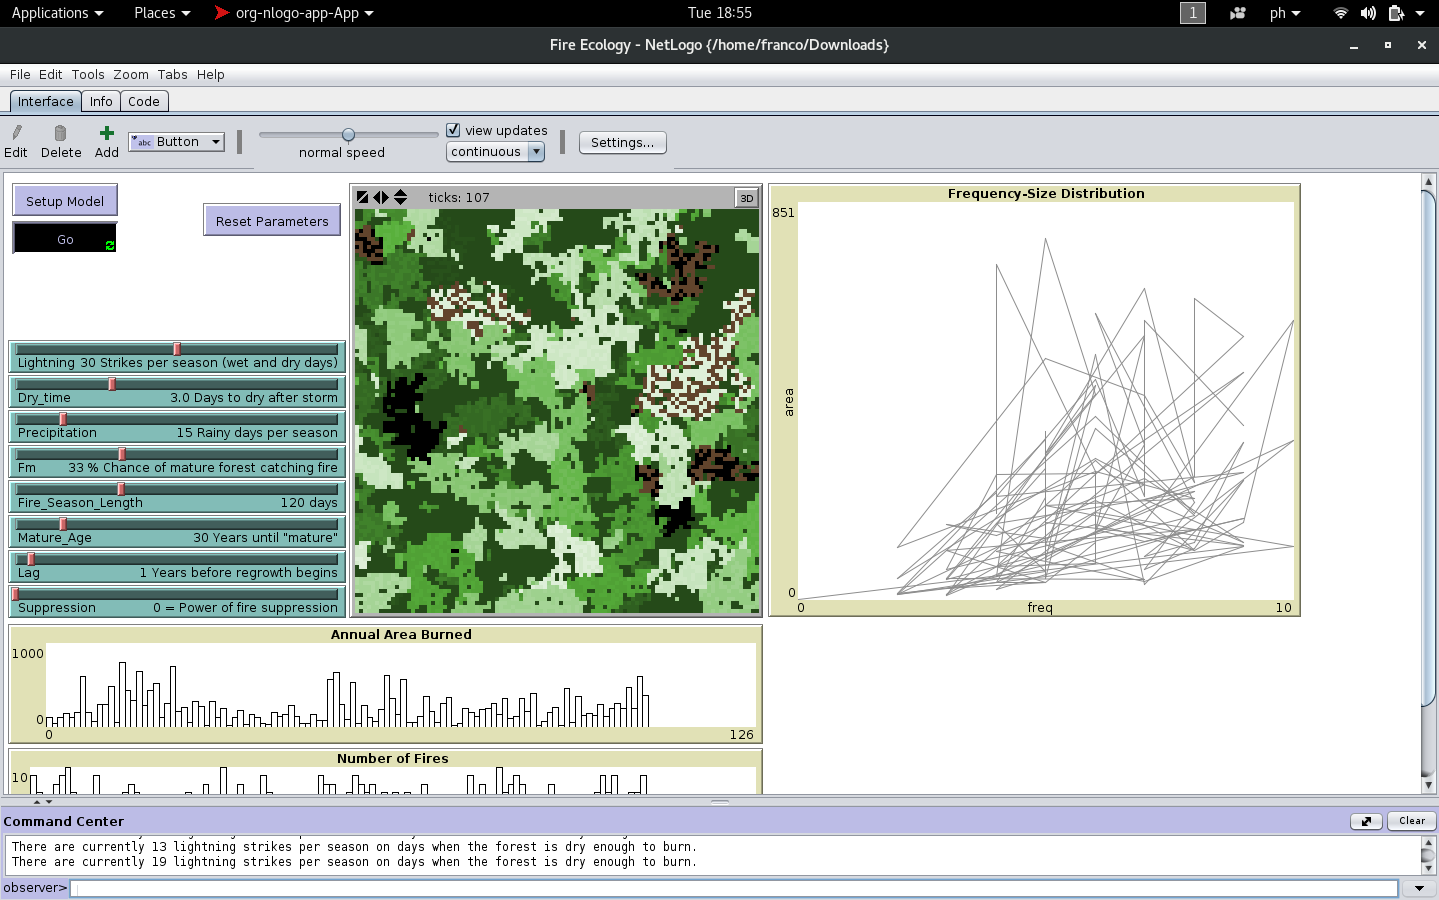
\includegraphics[width=1.5\textwidth]{first}
	\caption{Forest fires exhibiting fractal properties.}
\end{figure}
\end{landscape}

The graphs of annual area burned per time is aperiodic and does not go into infinity, same as the number of fires per time. A graph has been added (on the right side) to plot the fire frequency to area trajectory at each time $t$. Consequently, the graph stays on a fixed region and does not approach infinity.

\section{Immunizing a Forest}
For the model to include an immunity dynamic introducing parameter $g$ and modification of rule 5 in necessary such that "a green tree becomes a burning tree with probability $(1-g^n)$ if $n$ of its nearest neighbors is burning"\cite{bib:rest}. Otherwise it remains green. The parameter $g$ introduces a critical threshold $g^\star = 1.2$ above and fires will not occur effectively. The following modifications are included in the source code:

\begin{itemize}
	\item Adding a slider and a immunity parameter $g$. If $g=1$ then a tree is immune with probability 1.
	\item Modifying the boolean condition on the innermost \texttt{if} statement on the \texttt{spread} function to
	\begin{itemize}
		\item \texttt{if age != 0 [}
		\item \texttt{set j sum[count fires-here] of neighbors4}
		\item \texttt{set p (1 - g ** j)}
		\item \texttt{if random-float 1 < p [ignite]}
		\item \texttt{]}
	\end{itemize}
\end{itemize}

The figure below shows an 'immune' forest given $g=0.7$. Annual area burned is relatively low. The large graph on the right shows trajectory of area to frequency as time increases. Notice that after some time it approaches a certain attractor meaning the annual area burned is kept bounded, thus the forest is fire-immune.

\begin{landscape}
	\begin{figure}[H]
		\centering
		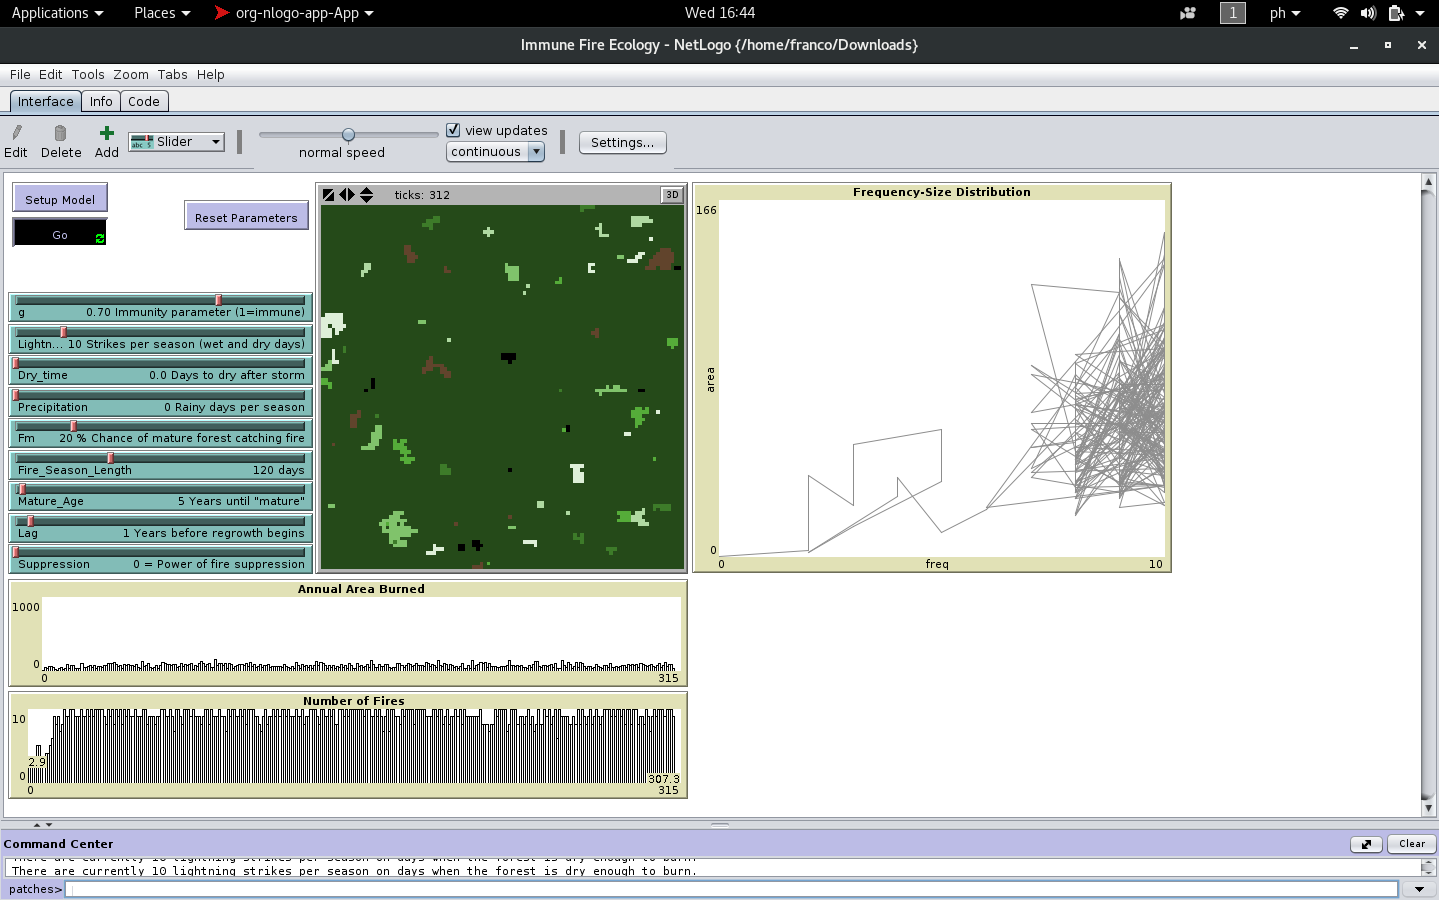
\includegraphics[width=1.5\textwidth]{second}
		\caption{Forest fires with immunity.}
	\end{figure}
\end{landscape}

\section{Self-organized Criticality}
From wiki, self-organized criticality is a property of dynamical systems where the critical or fixed point is an attractor. In the paper of \cite{bib:self}, a forest-fire leads to a self-organized critical state in the limit $f \rightarrow 0$ when the times scales of tree growth and burning down of clusters are separated.

In letting $f \rightarrow 0$ the number of lightning strikes and $f$ has set to a low value so that the time between two consecutive strikes per cell is very large. Mature age is set to 1 year before growth begins. In this manner, most of the forest will burn and mean density will be kept low as possible as in a critical state.

Again, the double separation of time scales has been observed in the simulation. In the netlogo simulation\cite{bib:model} parameters are set as follows in the screenshot below. 

\begin{landscape}
	\begin{figure}[H]
		\centering
		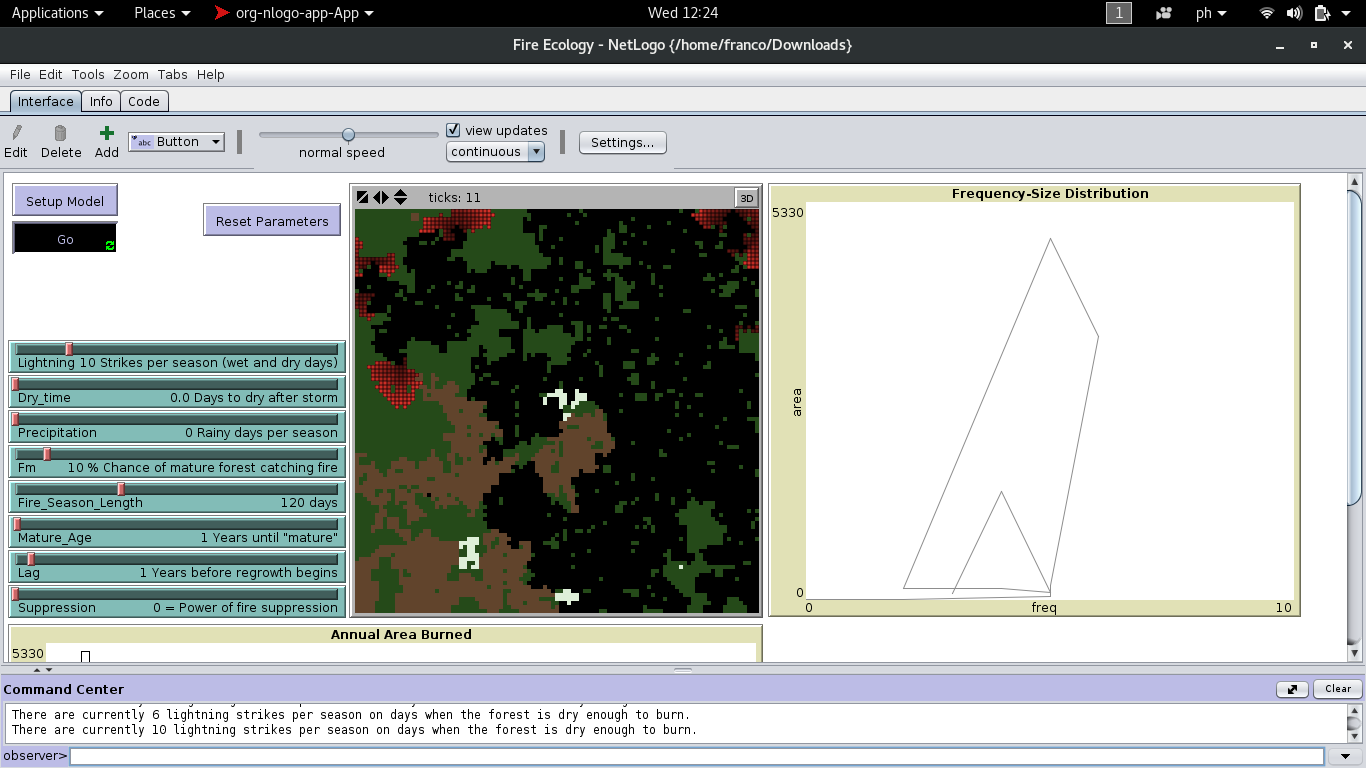
\includegraphics[width=1.5\textwidth]{third}
		\caption{Forest fires self-organizing critical state.}
	\end{figure}
\end{landscape}

\begin{thebibliography}{5}
	\bibitem{bib:model} R. Kelly, (2009). \emph{NetLogo Fire Ecology model.} Department of Plant Biology, University of Illinois, Urbana, IL. \url{http://ccl.northwestern.edu/netlogo/models/community/Fire\%20Ecology}
	
	\bibitem{bib:rest} M. Yoder, L. Turcotte, J. Rundle, (2011). \emph{Forest-fire model with natural fire resistance.} Department of Physics, University of California Davis.
	
	\bibitem{bib:self} B. Drossel and F. Schwabl (1992). \emph{Self-Organized Critical Forest-Fire Model}.
\end{thebibliography}
\end{document}